Heating scenario. Resulting plot of heat map. 
%TODO Make a diagram of how the data is processed. Flow chart? 
\subsubsection{Relative Humidity}
	Assuming no additional humidifiers, the resulting relative humidity inside an average household can be easily modelled by assuming constant humidity ratio heating through assumed processes as we have illustrated in the methodology. We can estimate the relative humidity of the corresponding area on continental United States, or as shown in Figure~\ref{fg:RHmap}. 

	\begin{figure}[h!]
	\centering
	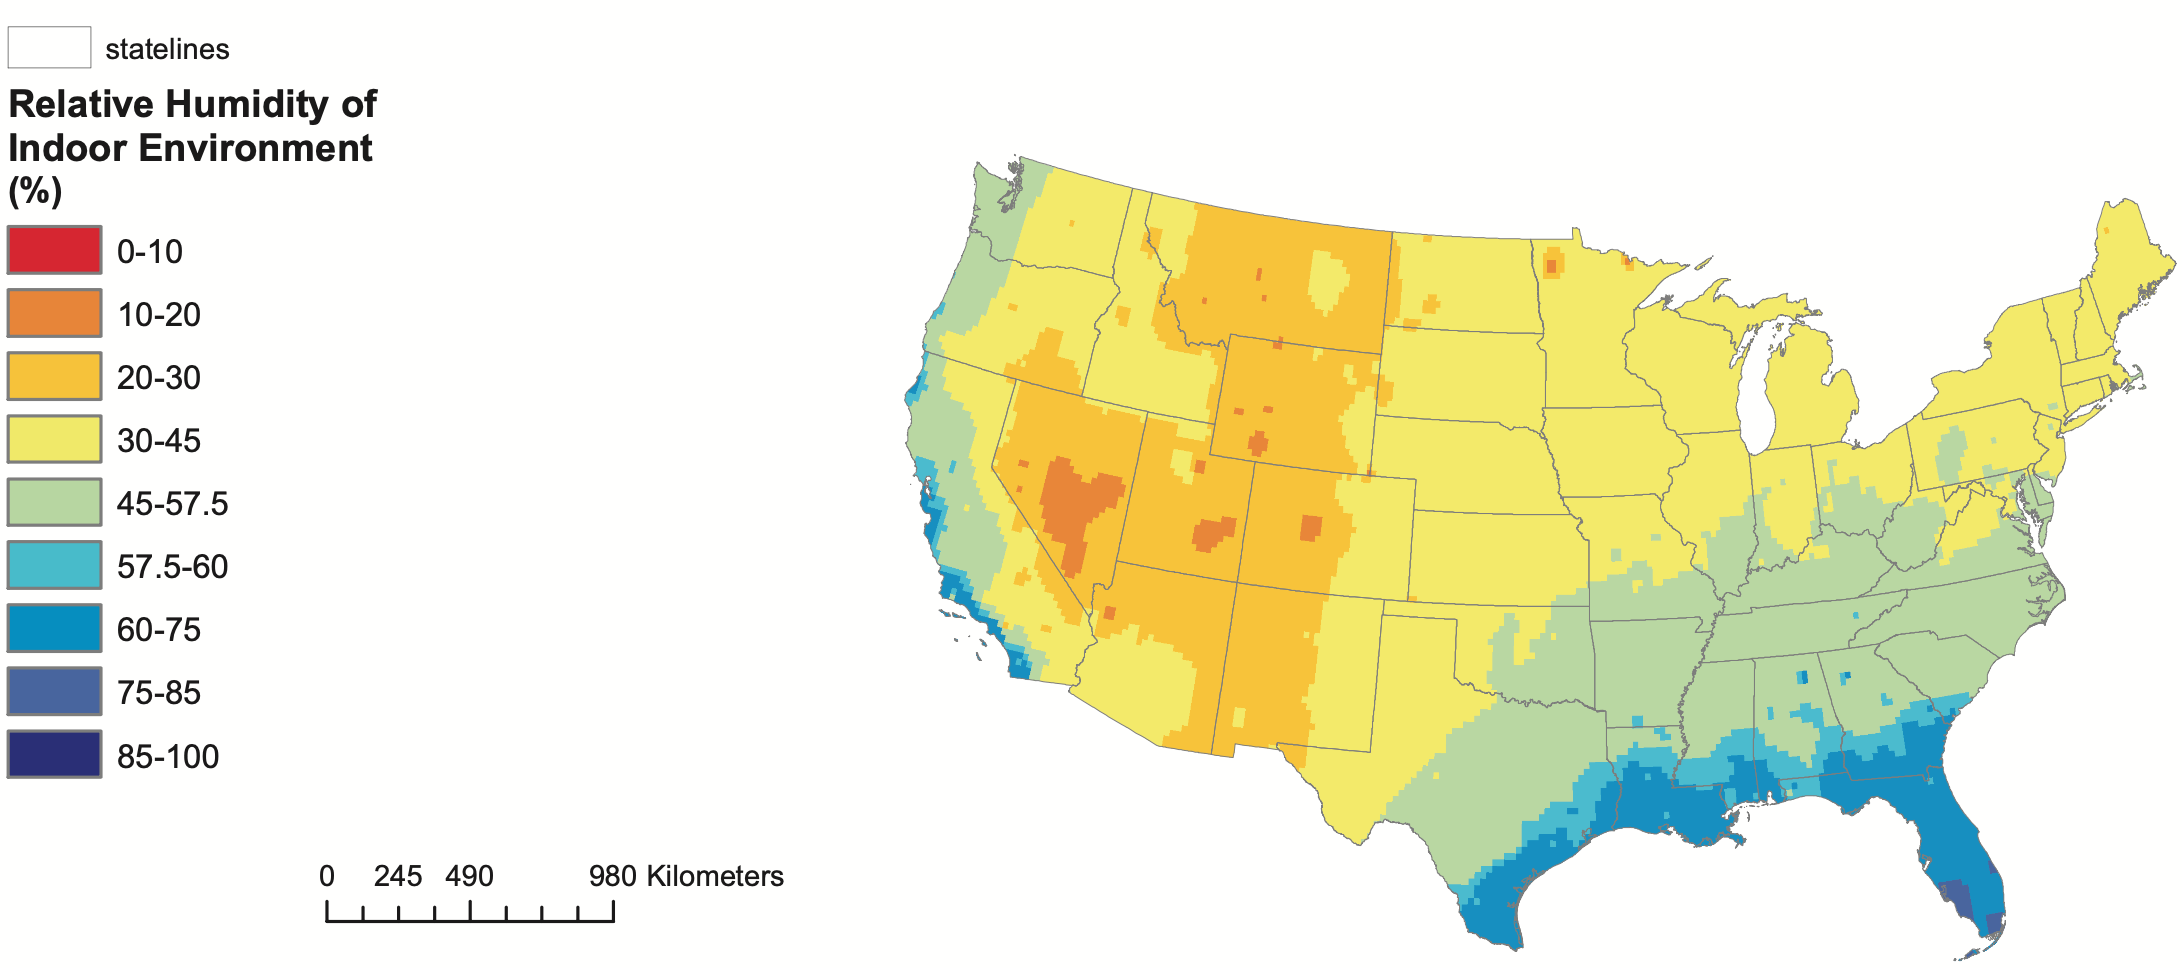
\includegraphics[width=0.7\textwidth]{heat62.png}\\
	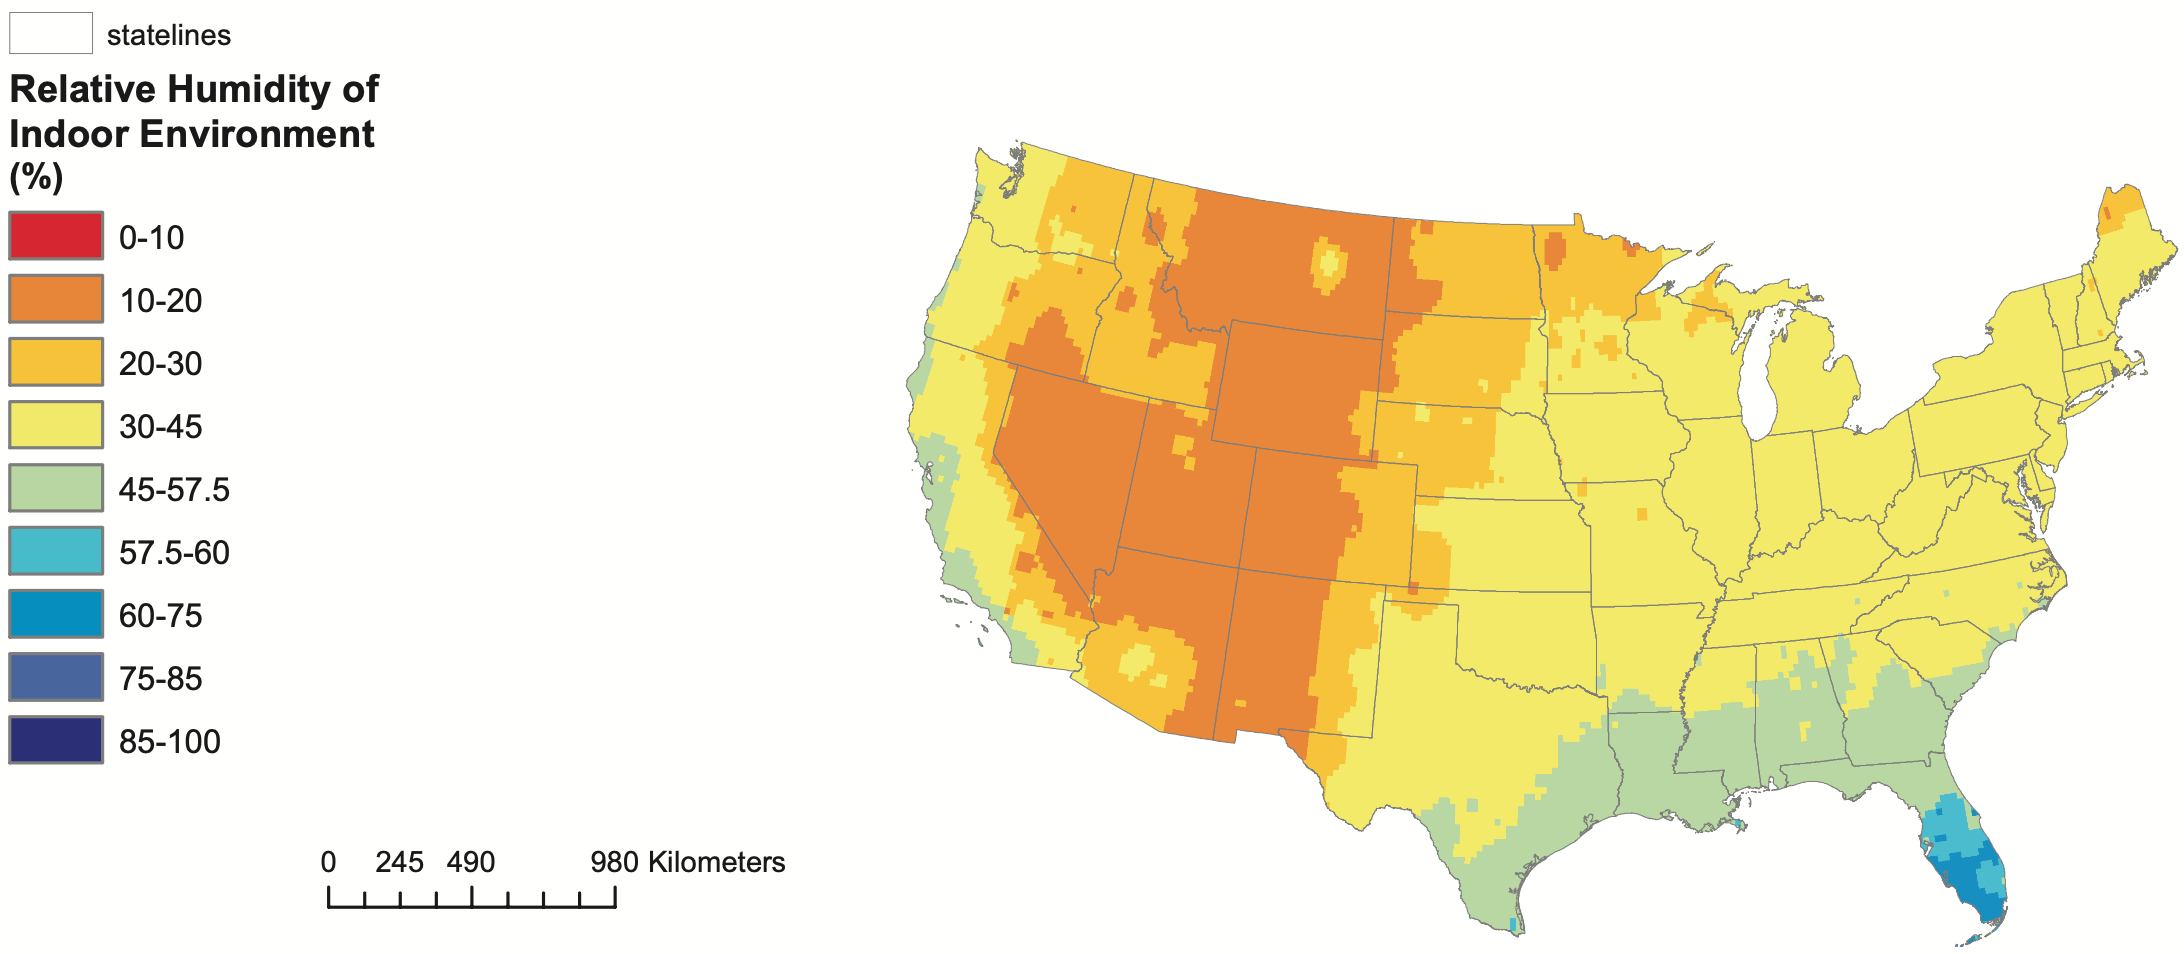
\includegraphics[width=0.7\textwidth]{heat68.png}\\
	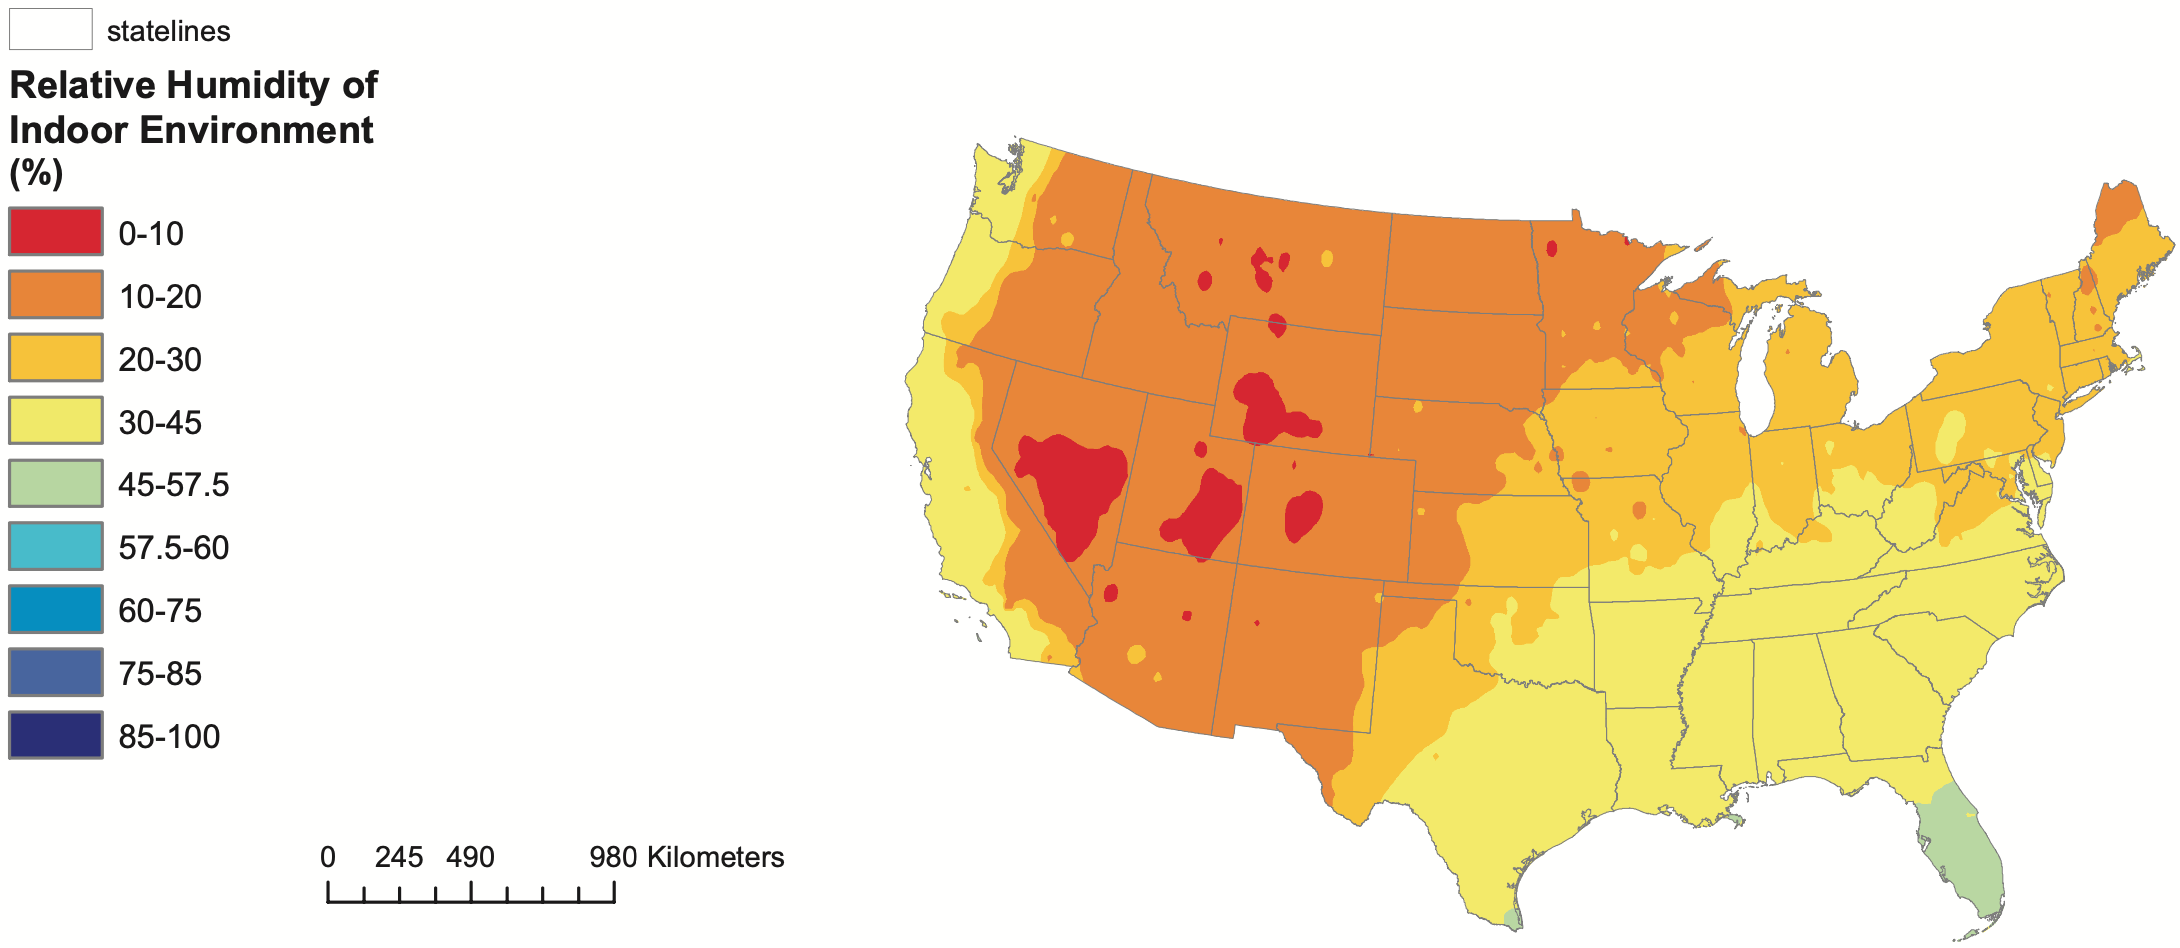
\includegraphics[width=0.7\textwidth]{heat74.png}\\
	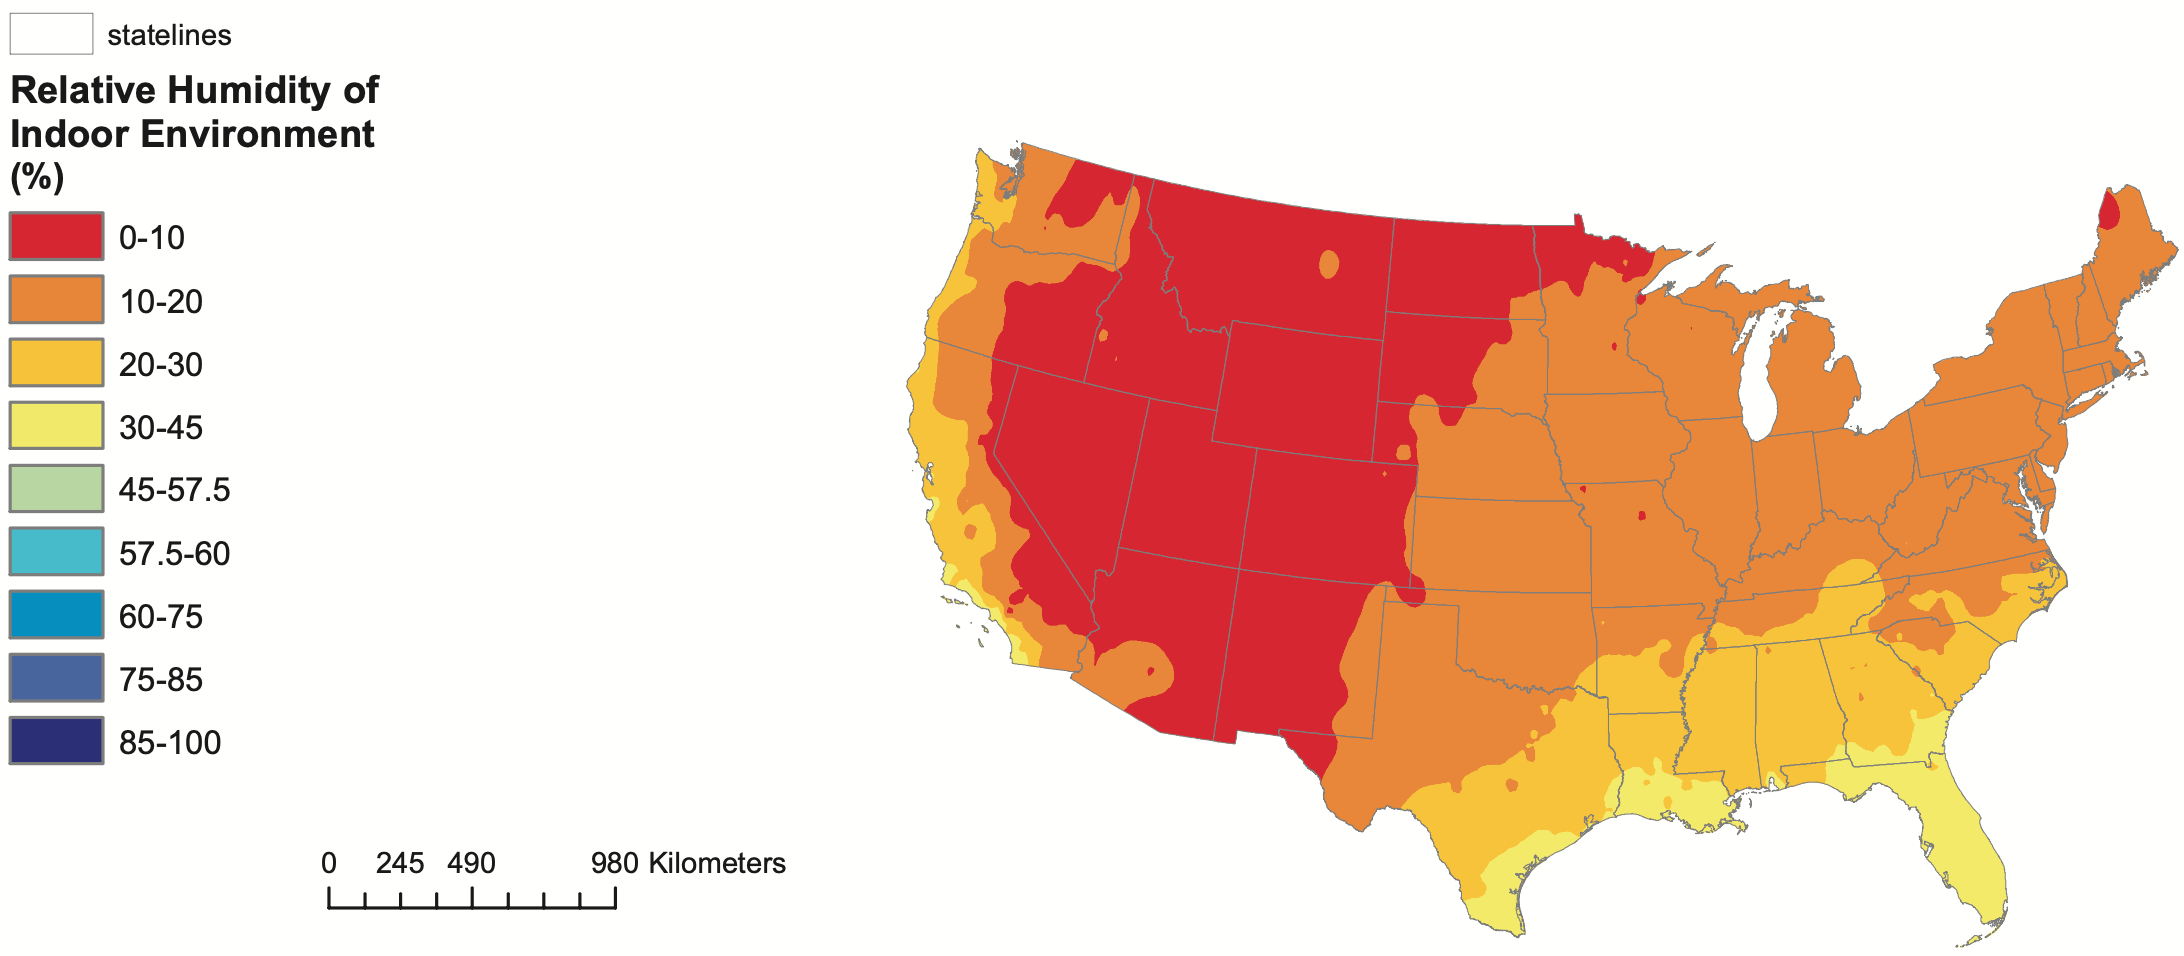
\includegraphics[width=0.7\textwidth]{heat80.png}
	\caption{Relative Humidity map generated for four different set points in Continental US.}\label{fg:RHmap}
	\end{figure}

	As we are only assuming the air undergoes a constant humidity ratio process of being sensibly heated up, the resulting heat map shown in Figure~\ref{fg:RHmap} is a very good indicator on how the set points may affect the relative humidity of an indoor environment without additional humidifiers added to the systems. From top to bottom, we plot the resulting relative humidity distribution for the four set points we selected previously, with the lowest heating set point (18 $\degree C$) on the top, and the highest set point temperature (26.7 $\degree C$) at the bottom. For the highest set point (80 $\degree F$, or 26.7 $\degree C$), an air-based system will obviously require additional humidifiers. This applies to the entire continental US, as the majority of country will result in an indoor humidity lower than the ASHARE mandate of 30\%. Using a lower set point temperature, in this case 20 and 23.3 $\degree C$, clearly improves the relative humidity of the indoor environment. However, there is still approximately 63.5\% of the entire country (weighted by area) that may have a relative humidity lower than the ASHRAE recommendation of 30\% for the set point of 23.3 $\degree C$. This number is lower for the set point of 20 $\degree C$ at 42.1\%, but still significant enough to raise concerns. Using a set point of 18 $\degree C$ appears to eliminate most of the humidification requirements, particularly for the midwest area in the continental US. However, the resulting RH distribution in the southeast area appears to create excessively high RH levels, which may suggest a higher set point for all-air system is more desirable.

	We also want to point out that the set point temperature here is not the equivalent of the supply air temperature. The set point temperature we are using is merely an indicator of the minimum amount of energy that needs to be delivered to ensure the state of the air. This psychrometric approach should not be confused with the actual energy demand of buildings, which will likely be much higher due to the infiltration, presence of the occupants, and other potential disturbances of an ideal indoor environment. 

\subsubsection{Energy Savings}
	To address the low RH problem in the residential homes when using all-air systems, an ideal solution will be to use humidifiers - which could help us investigate the energy implications when additional humidifiers are needed. Conversely speaking, this could also be considered energy savings potential from radiant systems, where a lower set point temperature is made possible at a higher relative humidity. 

	To provide a better quantitative comparison of the energy savings potentials, we will be comparing our results through the CDD and EDD calculations of the data files from selected major cities across all climate zones.

	\begin{figure}[h!]
	\centering
	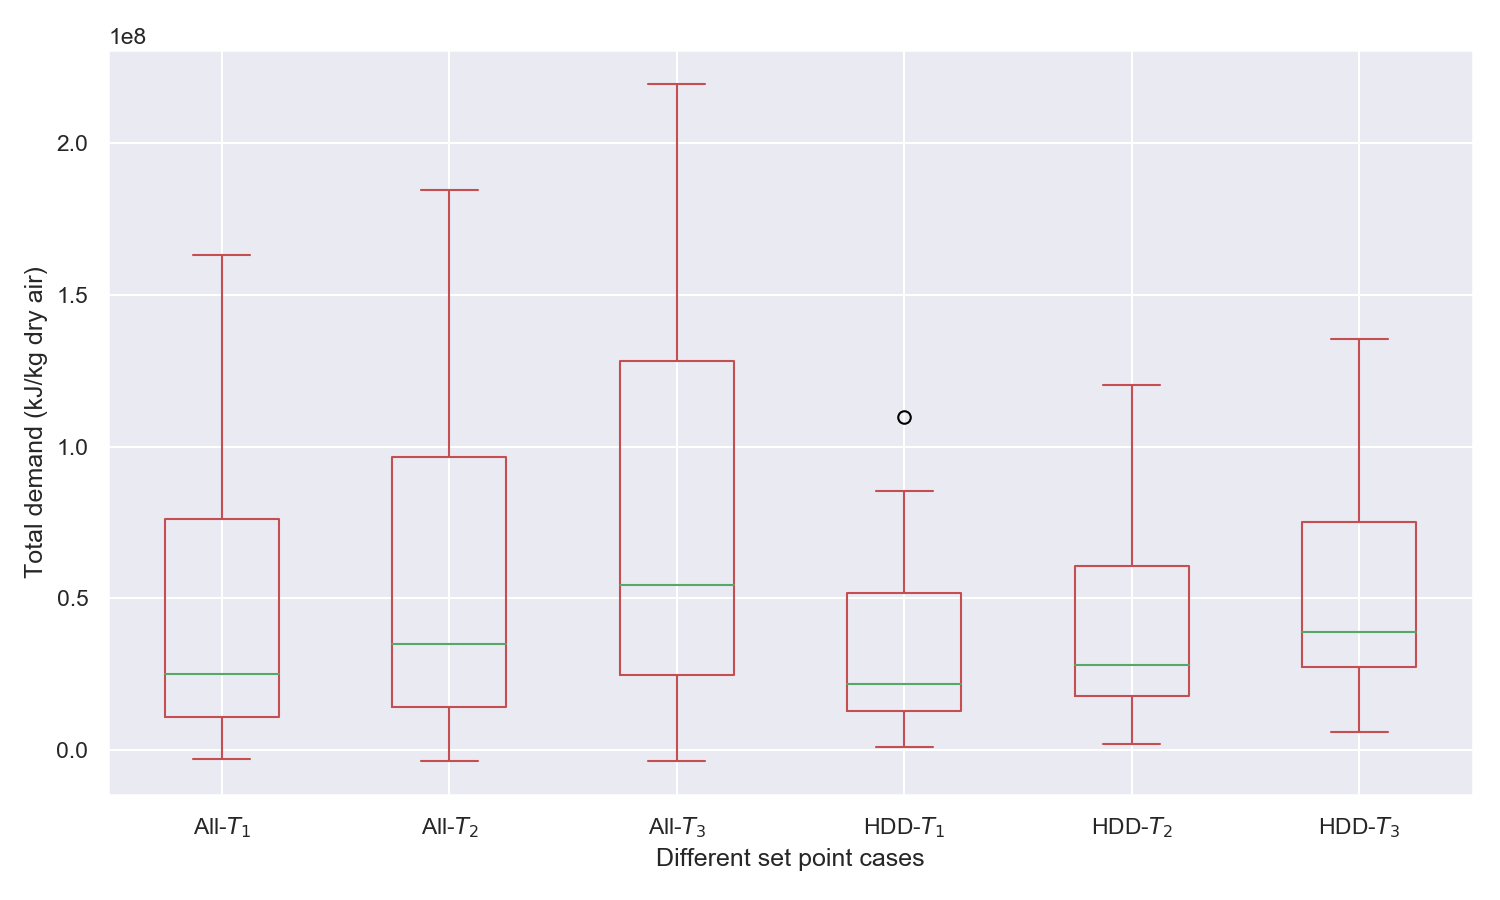
\includegraphics[width=0.8\textwidth]{boxheat.png}
	\caption{Box plot comparing the total energy demand from psychrometric analysis over dry-bulb only analysis}\label{fg:heatall}
	\end{figure}

	To visualize the overall energy demand change, we are plotting the overall demand and the corresponding heating degree day (sensible) demand in Figure~\ref{fg:heatall}. The influence on energy demand from the need to humidify the air is obvious, as the total demand increases when the set point increases from $T_1$ to $T_2$. However, the overall separation bewteen the different weather stations appears to widen. To better understand how this is affecting the different major cities through different climates, we have also plotted Figure~\ref{fg:heatcities} to illustrate how the additional energy necessray to humidify the air changes between different cities.

	\begin{figure}[h!]
	\centering
	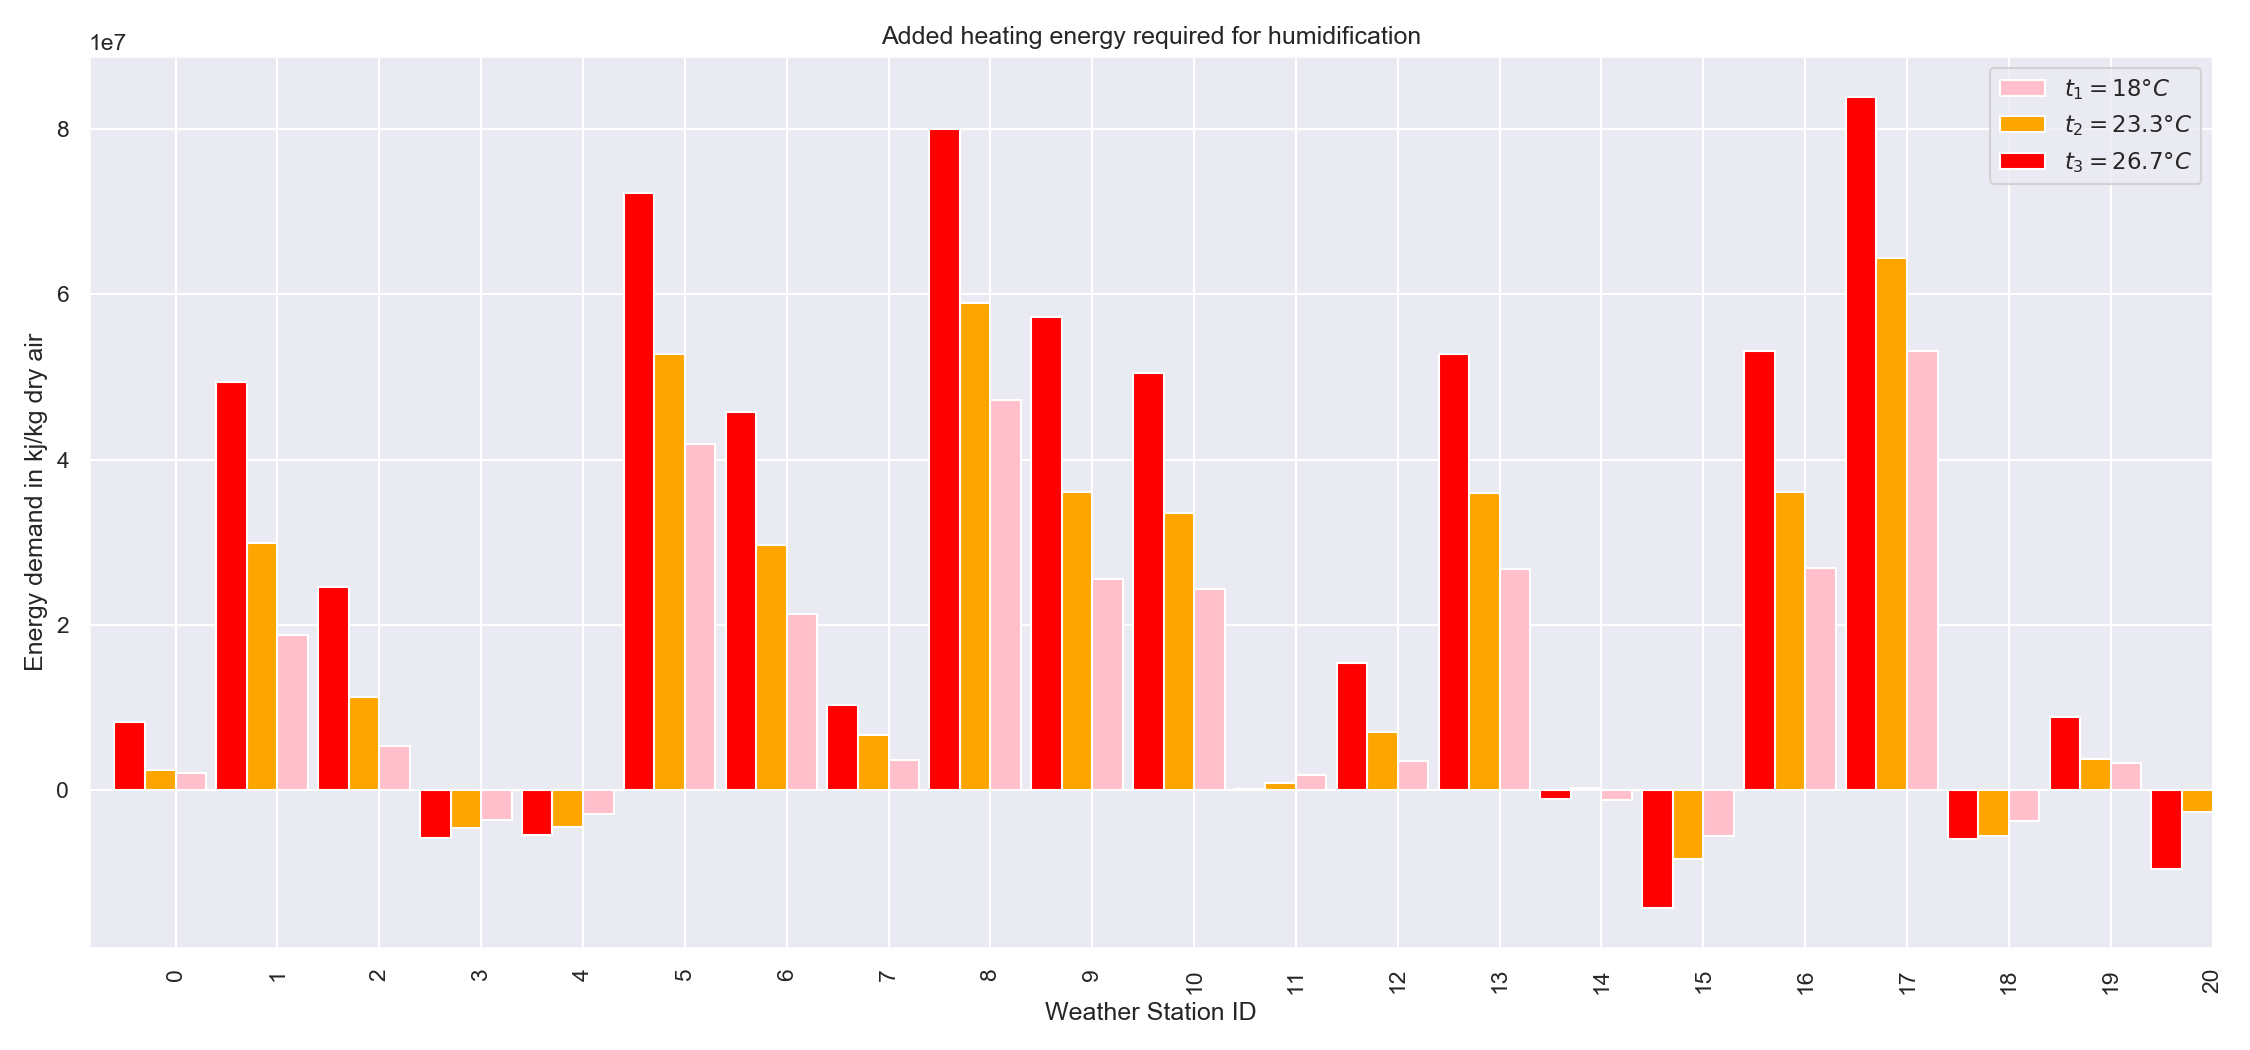
\includegraphics[width=0.8\textwidth]{heatsave.png}
	\caption{Box plot comparing the total energy demand from psychrometric analysis over dry-bulb only analysis}\label{fg:heatcities}
	\end{figure}

	According to Figure~\ref{fg:heatcities}, 71.4\% of all the stations we harvest data for will require energy to achieve at least 50\% humidity for the indoor environment. For cities in colder environments, the energy required to humidify the air could increase significantly when the set points are higher, ranging from 60\%  (Station ID=8) to up to 95\% (Station ID = 6). As our interests are primarily psychrometric-based, it is important to note that this does not reflect how different systems consumes and delivers said states of humid air, only how much energy needs to be delivered from the systems to the outdoor air to maintain a satisfying indoor environment. 